\documentclass{source/Report}

\major{地理信息科学}
\name{陈杰伟}
\title{RV64 内核线程调度}
\stuid{3200101205}
\college{地球科学学院}
\date{\today}
\lab{玉泉曹光彪-西503}
\course{操作系统}
\instructor{寿黎但}
\grades{}
\expname{RV64 内核线程调度}
\exptype{编程实验}
\partner{无}

\begin{document}
\makecover
\makeheader
\section{实验目的}
- 了解线程概念, 并学习线程相关结构体, 并实现线程的初始化功能。

- 了解如何使用时钟中断来实现线程的调度。

- 了解线程切换原理, 并实现线程的切换。

- 掌握简单的线程调度算法, 并完成两种简单调度算法的实现

\section{实验环境}
Ubuntu 20.04

\section{实验步骤}
\subsection{线程初始化}

在初始化线程的时候, 我们参考Linux v0.11中的实现为每个线程分配一个 4KB 的物理页, 我们将 task\_struct 存放在该页的低地址部分,  将线程的栈指针 sp 指向该页的高地址。    

OS run 起来的时候, 其本身就是一个线程 idle线程, 第一步为 idle 设置 task\_struct。并将 current, task[0] 都指向 idle。

将 task[1]~ task[NR\_TASKS - 1], 全部初始化,  这里和 idle 设置的区别在于要为这些线程设置 thread\_struct 中的 ra 和 sp.

\begin{lstlisting}[language = c, title = {线程初始化}]
    void task_init()
    {
        idle = (struct task_struct *)kalloc();
        // 调用 kalloc() 为 idle 分配一个物理页
    
        idle->state = TASK_RUNNING;
        // 设置 state 为 TASK_RUNNING;
    
        idle->counter = 0;
        idle->counter = PRIORITY_IDLE;
        // 由于 idle 不参与调度 可以将其 counter / priority 设置为 0
    
        idle->pid = 0;
        // 设置 idle 的 pid 为 0
    
        current = idle;
        task[0] = idle;
    
        // 为 task[1] ~ task[NR_TASKS - 1] 设置 thread_struct 中的 ra 和 sp,
        // 其中 ra 设置为 __dummy的地址,  sp 设置为 该线程申请的物理页的高地址
    
        int i = 0;
        for (i = 1; i < NR_TASKS; ++i)
        {
            task[i] = (struct task_struct *)kalloc();
    
            task[i]->state = TASK_RUNNING;
    
            task[i]->counter = 0;
            task[i]->priority = rand();
    
            task[i]->pid = i;
    
            task[i]->thread.ra = (uint64)&__dummy;
            task[i]->thread.sp = (uint64)task[i] + PGSIZE;
        }
    
        printk("...proc_init done!\n");
        printk("Hello RISC-V\n");
        printk("idle process is running!\n");
        printk("\n");
    
        reset_thread();
    
        return;
    }
\end{lstlisting}


\subsection{在 entry.S 添加 \_\_dummy}

当线程在运行时, 由于时钟中断的触发, 会将当前运行线程的上下文环境保存在栈上。当线程再次被调度时, 会将上下文从栈上恢复, 但是当创建一个新的线程, 此时线程的栈为空, 当这个线程被调度时, 是没有上下文需要被恢复的, 所以需要为线程第一次调度提供一个特殊的返回函数 \_\_dummy

在\_\_dummy 中将 sepc 设置为\ dummy() 的地址, 并使用 sret 从中断中返回。

\begin{lstlisting}[language = bash, title = {\_\_dummy}]
    __dummy:
    la t0, dummy
    csrw sepc, t0
    sret
\end{lstlisting}

\subsection{实现调度入口函数}

实现 do\_timer(), 并在 时钟中断处理函数 中调用。    

\begin{lstlisting}[language = c, title = {do\_timer}]
    void do_timer(void)
    {
        // 如果当前线程是 idle 线程 直接进行调度
        if (current->pid == 0)
            schedule();
    
        // 如果当前线程不是 idle 对当前线程的运行剩余时间减1 若剩余时间仍然大于0 则直接返回 否则进行调度
        else
        {
            current->counter--;
            if (current->counter > 0)
                return;
            else
                schedule();
        }
        return;
    }
\end{lstlisting}


\subsection{实现线程切换}

在 entry.S 中实现线程上下文切换 \_\_switch\_to:

- \_\_switch\_to接受两个 task\_struct 指针作为参数

- 保存当前线程的ra, sp, s0~s11到当前线程的 thread\_struct 中

- 将下一个线程的 thread\_struct 中的相关数据载入到ra, sp, s0~s11中。

- 同时要在汇编中改变current指针所指向的地址,这样在sret触发时钟中断后不会重新再进入调度函数

\begin{lstlisting}[language = bash, title = {\_\_switch\_to}]
    .globl __switch_to
__switch_to:
    # save state to prev process
    sd ra, 8*5(a0)
    sd sp, 8*6(a0)
    sd s0, 8*7(a0)
    sd s1, 8*8(a0)
    sd s2, 8*9(a0)
    sd s3, 8*10(a0)
    sd s4, 8*11(a0)
    sd s5, 8*12(a0)
    sd s6, 8*13(a0)
    sd s7, 8*14(a0)
    sd s8, 8*15(a0)
    sd s9, 8*16(a0)
    sd s10, 8*17(a0)
    sd s11, 8*18(a0)

    # restore state from next process
    ld ra, 8*5(a1)
    ld sp, 8*6(a1)
    ld s0, 8*7(a1)
    ld s1, 8*8(a1)
    ld s2, 8*9(a1)
    ld s3, 8*10(a1)
    ld s4, 8*11(a1)
    ld s5, 8*12(a1)
    ld s6, 8*13(a1)
    ld s7, 8*14(a1)
    ld s8, 8*15(a1)
    ld s9, 8*16(a1)
    ld s10, 8*17(a1)
    ld s11, 8*18(a1)

    #指针移动
    la t0, current
    sd a1, 0(t0)

    ret
\end{lstlisting}

\subsection{短作业优先调度算法}

当需要进行调度时按照一下规则进行调度:

- 遍历线程指针数组task(不包括 idle , 即 task[0] ), 在所有运行状态 (TASK\_RUNNING) 下的线程运行剩余时间最少的线程作为下一个执行的线程。

- 如果所有运行状态下的线程运行剩余时间都为0, 则对 task[1] ~ task[NR\_TASKS-1] 的运行剩余时间重新赋值 (使用 rand()) , 之后再重新进行调度。

\begin{lstlisting}[language = c, title = {短作业}]
    void schedule(void)
    {
        int i = 0;
        int to_execute = -1;
    
        int to_reset = 1;
    
        for (i = 1; i < NR_TASKS; i++)
        {
            if (task[i]->state != TASK_RUNNING)
                continue;
            if (task[i]->counter > 0)
                to_reset = 0;
            else
                continue;
            if (to_execute == -1 || task[i]->counter < task[to_execute]->counter)
                to_execute = i;
        }
    
        if (to_reset == 1)
        {
            reset_thread();
            schedule();
            return;
        }
    
        switch_to(task[to_execute]);
    
        return;
    }
\end{lstlisting}

\subsection{优先级调度算法}

参考 Linux v0.11 调度算法实现实现。   

\begin{lstlisting}[language = c, title = {优先级}]
    void schedule(void)
    {
        int i, next, c;
        struct task_struct **p;
    
        c = -1;
        next = 0;
        i = NR_TASKS;
        p = &task[NR_TASKS];
    
        while (--i)
        {
            if (!*--p)
                continue;
            if (((*p)->state == TASK_RUNNING) && ((int)(*p)->counter > c))
            {
                c = (*p)->counter;
                next = i;
            }
        }
    
        if (!c)
        {
            reset_thread();
            schedule();
            return;
        }
    
        switch_to(task[next]);
        return;
    }
\end{lstlisting}

\subsection{运行结果}

短作业调度算法结果如图1,能正确进行切换并读取保存上下文

\begin{figure}[p]
    \centering
    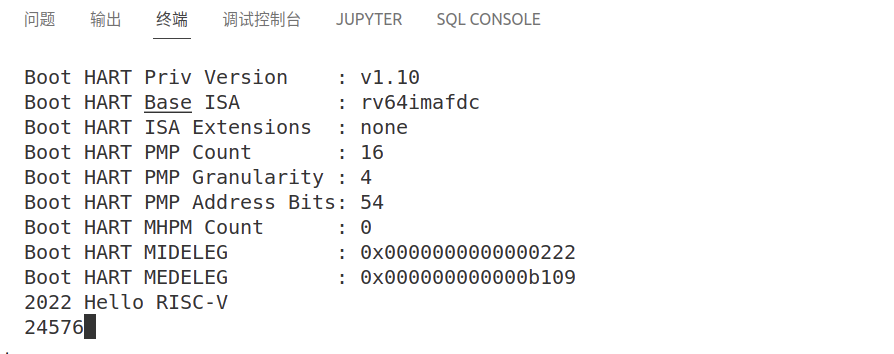
\includegraphics[width = 1\textwidth]{7}
    \caption{短作业结果}
\end{figure}

优先级调度算法结果如图2,能正确进行切换并读取保存上下文

\begin{figure}[p]
    \centering
    
\includegraphics[width = 1\textwidth]{8}
    \caption{优先级结果}
\end{figure}


\section{思考题}

1.在 RV64 中一共用 32 个通用寄存器, 为什么 context\_switch 中只保存了14个?

sp指示了线程运行栈的位置

ra代表了线程所执行函数的地址

sp, ra, s0-s11是Callee, 保存了线程当前的执行状态,而剩下的寄存器都是Caller,其中保存的信息在函数执行过程中可变,并没有必要将其存储到栈中

2. 当线程第一次调用时, 其 ra 所代表的返回点是 \_\_dummy。那么在之后的线程调用中 context\_switch 中, ra保存/恢复的函数返回点是什么呢? 请同学用 gdb 尝试追踪一次完整的线程切换流程, 并关注每一次 ra 的变换 (需要截图)。

第一次调用时ra保存值为\_\_dummy的地址如图3,

\begin{figure}[p]
    \centering
    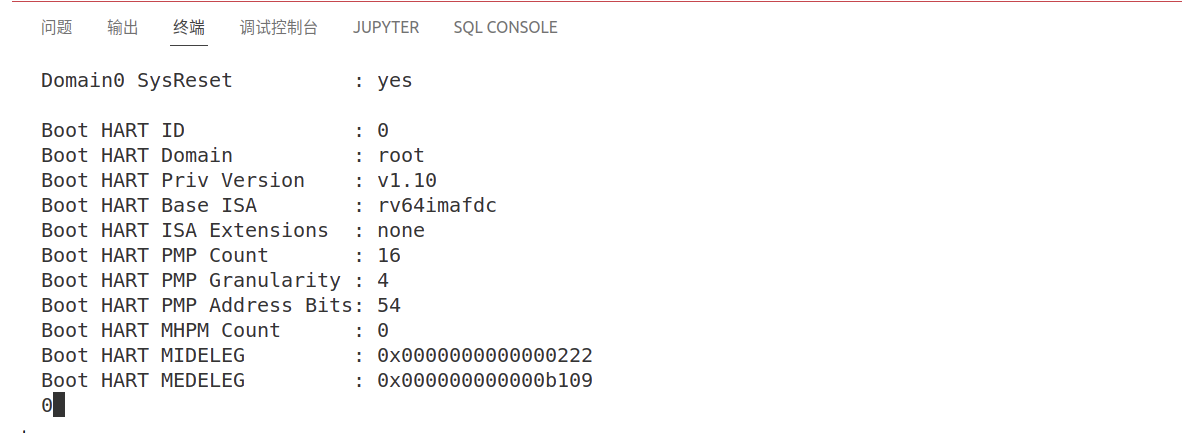
\includegraphics[width = 1\textwidth]{3}
    \caption{第一次ra}
\end{figure}

之后调用时保存的是自己正在执行的任务,即dummy函数中循环的地址,如图4

\begin{figure}[p]
    \centering
    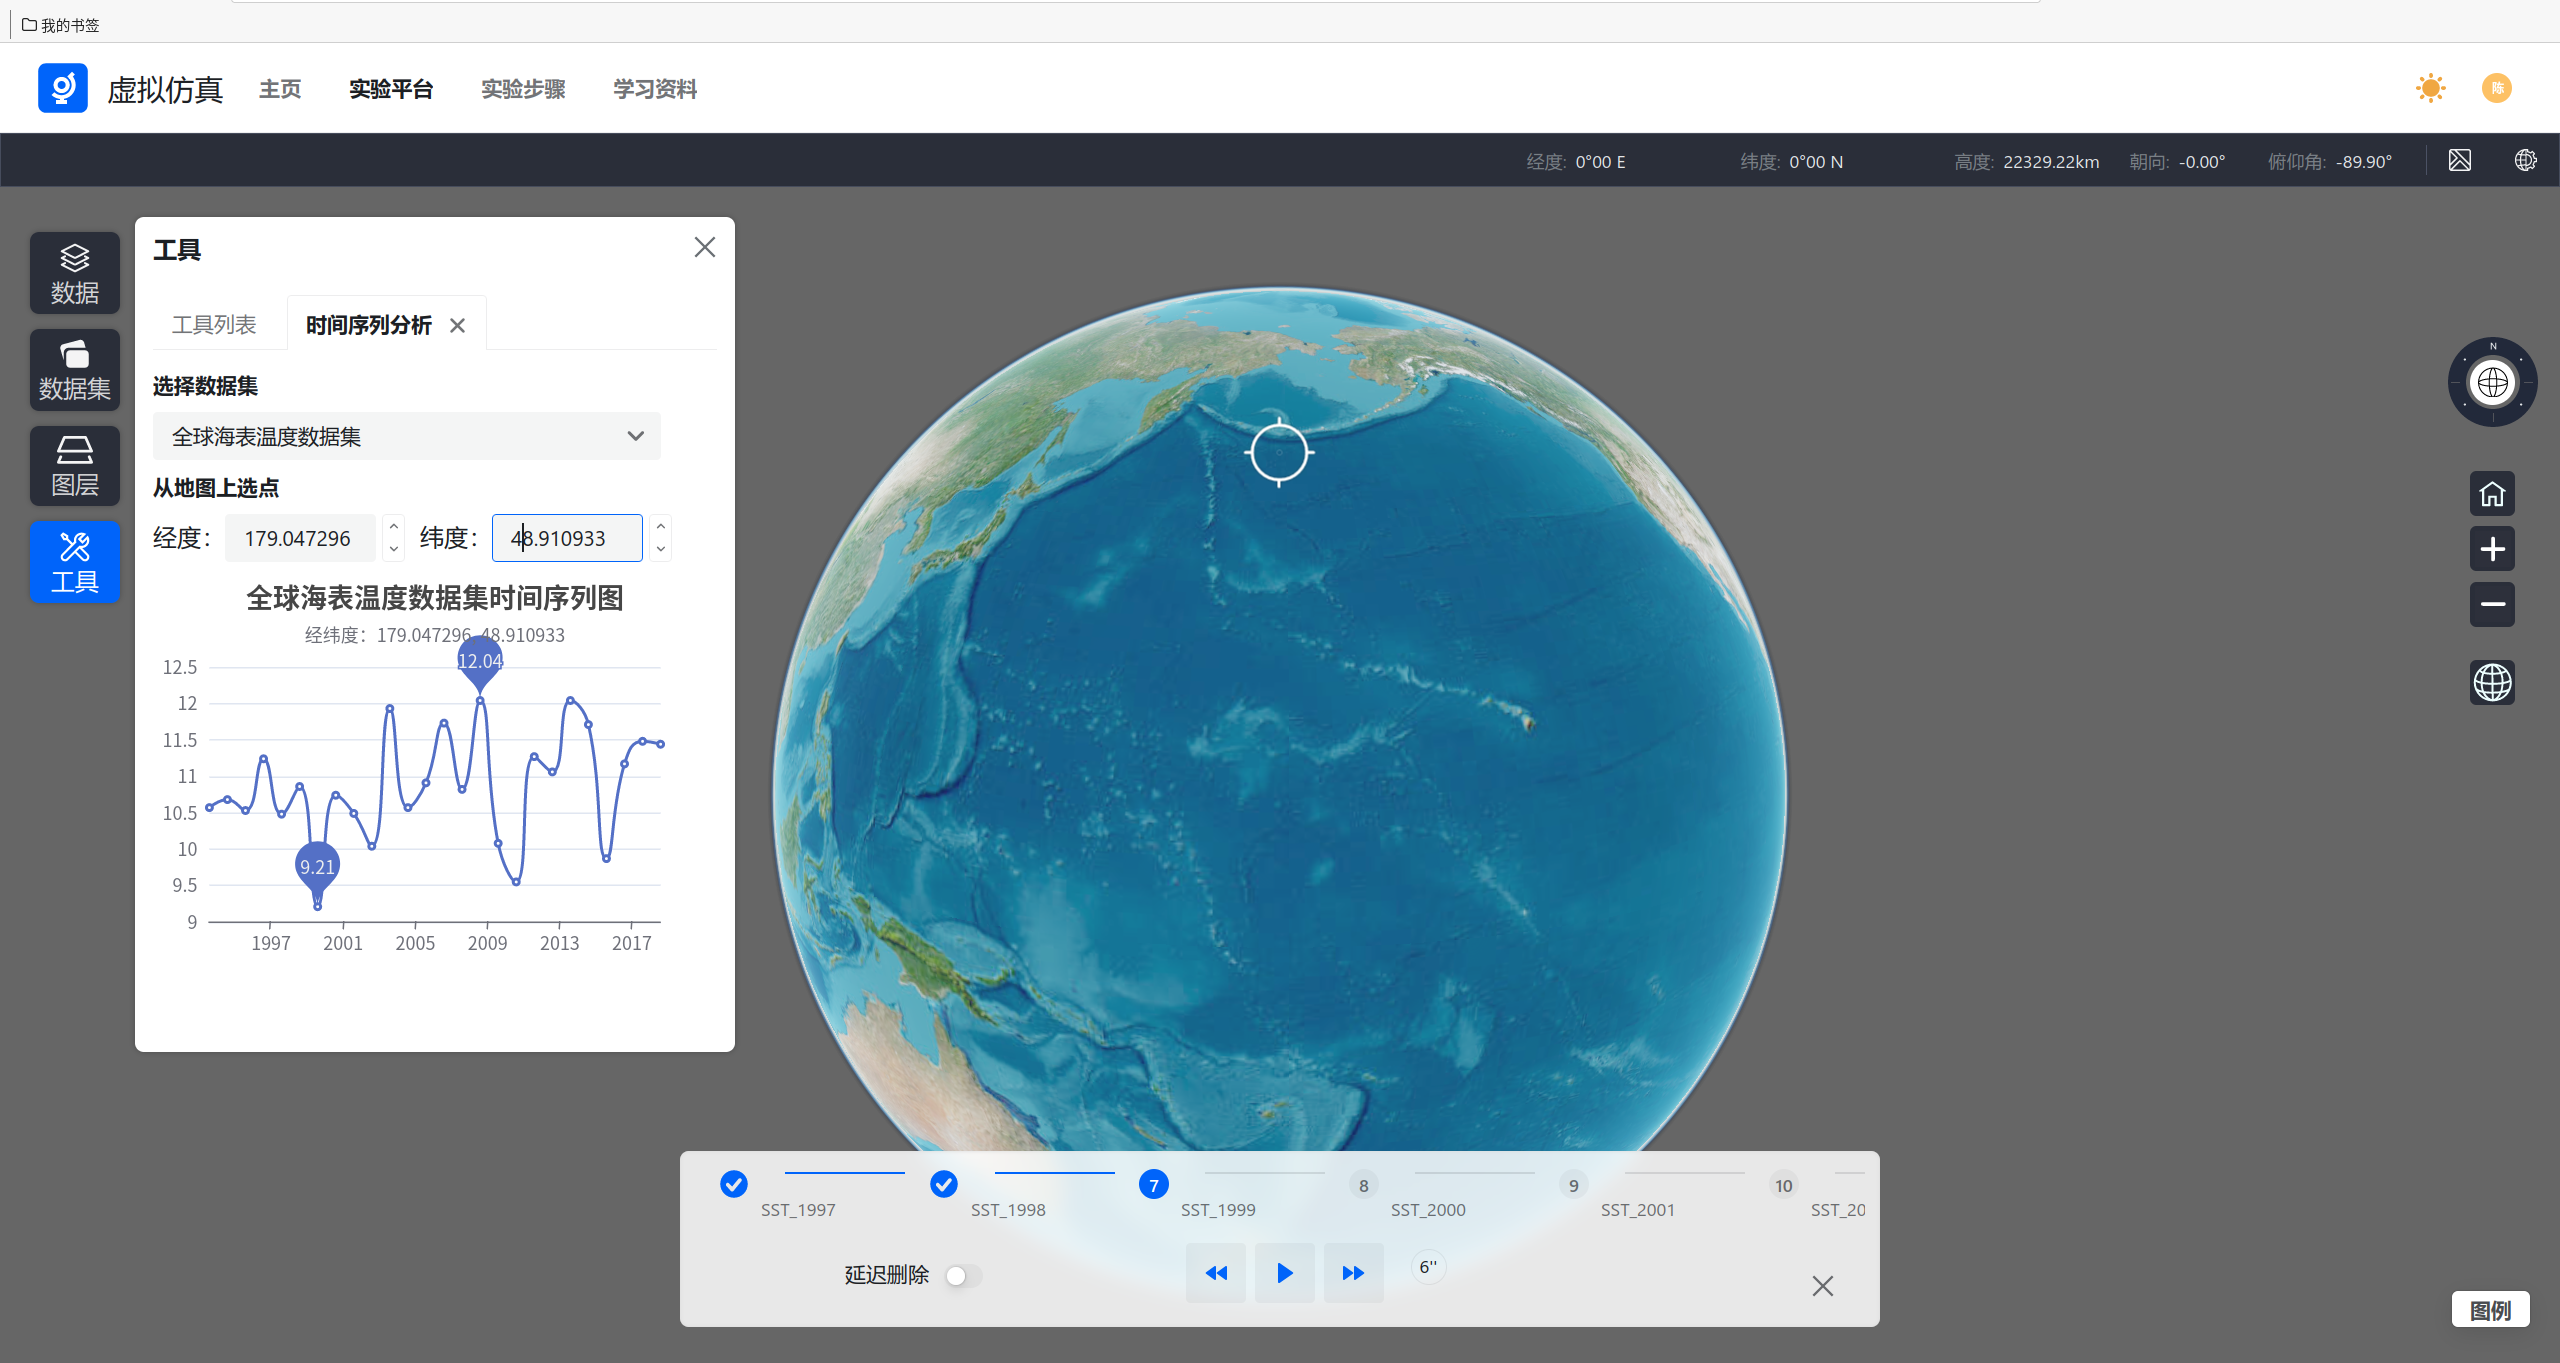
\includegraphics[width = 1\textwidth]{6}
    \caption{之后ra}
\end{figure}


\end{document}

